
\numberwithin{equation}{section}
\numberwithin{figure}{section}
\numberwithin{table}{section}

Pipe buckling is expected to be one of the main sources of pipe failure because of the weakness of the pipe provided by DSATS \cite{dsats} and reports from previous contests. The drill string will therefore be designed to address this issue and thus limit the risk of buckling.

Buckling occurs when too much weight is applied at the top of the drill string. This puts the pipe in a state of compression where it starts bending and becomes prone to increased metal fatigue failure. Furthermore, the body of the drill pipe wears rapidly due to abrasion along the wall. The worst-case scenario is that the pipe fails because of buckling.

This phenomenon can be prevented by increasing the tension of the drill string and thus avoiding entering a state of compression. There are two ways to achieve this, one is to reduce the weight applied at the top and the other is to increase the weight in the lower part of the string.

Although reducing the weight applied by the top drive is a simple and effective solution, it will limit the amount of weight applied on the bit and thus slow down the drilling speed. Increasing the weight in the bottom hole assembly (BHA) has therefore been chosen as the best solution.

In the industry, the weight of the BHA is increased by adding drill collars and heavy-weight drill pipes. The scale of this project makes it difficult to add sufficient weight in this manner. The proposed solution is therefore to increase the tension in the pipe wall by increasing the internal pressure of the pipe. This will be achieved by adding a nozzle in the BHA which means that the increase in internal pressure will result in a force, $F_c$, acting downwards on the constriction area. 

The sum of the weight of the drill string and the force $F_c$ will define the limit of the weight applied by the top drive. This will also enable the estimation of the required diameter of constriction.

\subsection{Weight of Drill String}
    
The weight of the drill pipe may be estimated using equation (\ref{eq:masscollar}).

\begin{equation}
\centering
   m_{DP}= \frac{\pi}{4} (d_o^2-d_i^2) \rho_{al} L
\label{eq:masscollar}
\end{equation}

$m_{DP}$ is the total mass of the drill pipe (kg), $d_o is$ the outer diameter of the drill pipe (m), $d_i$ is the inner diameter of the drill pipe (m), $\rho_{al}$ is the density of the aluminum (kg/m$^3$) and L is the length of the pipe (m).

The outer diameter of the drill pipe is 9.53 mm, the inner diameter is 7.75 mm, the density of aluminum is assumed to be 2,750 kg/m$^3$, and the length is 91.4 cm. This gives a total drill pipe weight of 0.061 kg.

The weight of the BHA is 0.227 kg and the weight of the bit is 0.300 kg. These weights may be altered during phase II. The total weight of the drill string is therefore 0.588 kg.

The buoyed weight of the string can be calculated using \ref{eq:buoyedweight}.

\begin{equation}
\centering
   m_{B}= m_{DP}(1-\frac{\rho_{w}}{\rho_{al}})+(m_{BHA}+m_{bit})(1-\frac{\rho_{w}}{\rho_{steel}})
\label{eq:buoyedweight}
\end{equation}

The density of steel is assumed to be 7,750 kg/m$^3$. This results in a total buoyed weight of 0.498 kg.

\subsection{Magnitude of Force F$_c$}
Through the following calculations, the magnitude of F$_c$ will be determined to be able to estimate how much weight can be applied through the top drive without putting the drill pipe in a state of compression. An illustration of this is shown in figure \ref{fig:strekkstring}.

\begin{figure} [H]
\centering
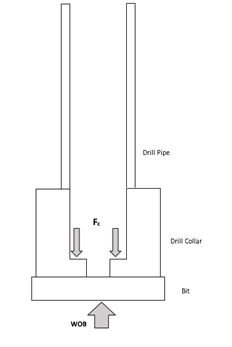
\includegraphics[width=0.5\textwidth]{figures/strekkstring.png}
\caption{Illustration of force F$_c$ counteracting the WOB and increasing the tension in the drill pipe wall}
\label{fig:strekkstring}
\end{figure}

The first step will be to calculate the burst pressure of the pipe as it is the limiting factor of the system. An estimate of the different pressure loss components in the circulation system will then make it possible to estimate the maximum value of $F_c$ and the maximum pump pressure. Finally, estimating the pressure drop over the constriction will enable the dimensioning of the constriction.

\subsubsection{Burst Pressure} \label{sssec:burst}
The limiting factor of the system is the risk of burst in the aluminum drill pipe. The increase in internal pressure inside the pipe causes an increase in differential pressure over the pipe wall which could lead to burst. Barlow’s formula, equation \ref{eq:barlow}, will be used to determine the ultimate burst pressure. 

\begin{equation}
\centering
   p_{br}=0.8 \frac{2 \sigma_{ys} t}{d_o}
\label{eq:barlow}
\end{equation}

$p_{br}$  is the maximum internal pressure the pipe can withstand (Pa), $\sigma_{ys}$ is the yield strength of aluminum (Pa), $t$ is the wall thickness of the pipe (m) and $d_o$ is the outer diameter of the pipe (m).

The yield strength of aluminum has been assumed to be 96.5 MPa, the safety factor has been chosen as 3, but may be changed during the construction phase, the thickness of the pipe wall is 0.89 mm and the outer diameter of the pipe is 9.53 mm. The burst pressure of the drill pipe has been estimated to be 5.26 MPa.

\subsubsection{Pressure Loss in Circulation System} \label{sssec:pressureloss}
The main purpose of the circulation system of this drilling rig is to provide additional internal pressure in the drill pipe to increase its geometric stiffness and reduce the risk of buckling. In addition to this, the circulation system will facilitate the removal of cuttings, cool and lubricate the drill string and bit, as well as provide well control through hydrostatic pressure. 

Fresh water was selected as drilling fluid to enable the circulation of cuttings out of the well. The use of mineral oil was considered, but due to the limited distance of transportation and the expected low pore pressure, it was concluded that fresh water was a better choice. This is a cheaper and more accessible alternative to standard drilling muds used in the industry.

\begin{figure} [H]
\centering
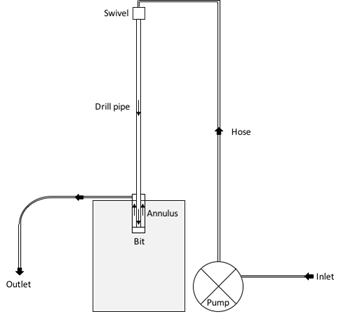
\includegraphics[width=0.5\textwidth]{figures/fluidsystem.png}
\caption{Illustration of the circulation system consisting of a mud pump, hose, swivel, drill pipe, BHA, bit nozzles and flowline.}
\label{fig:fluidsystem}
\end{figure}

A pump will be installed to both circulate the drilling fluid through the system and increase the internal pressure of the drill string. The recirculation of drilling fluid is not included in this design as it requires an advanced solid removal system. The fluid will be conducted out of the well and into a separate tank for storage. 

A density of 998.2 kg/m3 and dynamic viscosity of 0.001002 Pa·s have been used in the pressure loss calculations. This is based on the properties of water at a temperature of 20\degree C \cite{engtool}.

The fluid velocity through the different components was determined based on the minimum required flow velocity in the annulus to circulate the cuttings out of the well. It has been decided that the flow rate will be maintained constant during the drilling operation.

\paragraph{Fluid Flow Velocity}
To remove cuttings from the wellbore, the annular velocity must be greater than the cutting slip velocity. The cutting slip velocity is given by equation (\ref{eq:vsl}) which is valid for all Reynold’s numbers \cite{bourg}.

\begin{equation}
\centering
   v_{sl}= \sqrt{\frac{d_s}{f} \frac{(\rho_s-\rho_f)}{\rho_f}}
\label{eq:vsl}
\end{equation}

$d_s$ is the particle diameter (m), $\rho_s$ is the solid density (kg/m3), $\rho_f$ is the fluid density (kg/m3) and $f$ is the friction factor.

The maximum particle diameter was in this case assumed to be half the distance between the borehole wall and the outer diameter of the BHA, resulting in a particle diameter of 0.7 mm. The solid density was assumed to be 2,640 kg/m3 (based on density of granite). The friction factor $f$ can be estimated using an empirical relationship between Re, the sphere diameter and the sphericity. Because Re is dependent on the unknown slip velocity, an initial simplifying assumption must be made. To calculate the initial Reynold’s number, the slip velocity $v_sl$ will be approximated by Stokes’ relation for creeping flow around a spherical particle given by equation (\ref{eq:stoke}) \cite{bourg}.

\begin{equation}
\centering
   v_{sl}= \frac{d_s^2 (\rho_s-\rho_f)}{\mu}
\label{eq:stoke}
\end{equation}

The initial guess for the particle slip velocity is 0.42 m/s. Re can now be calculated based on the input data and the particle slip friction factor can then be estimated based on the empirical friction factor chart \cite{bourg}. Assuming a sphericity factor of 1, the friction factor is expected to be 0.6. This results in a cutting slip velocity of 0.16 m/s. Iterations were then performed until a good approximation was found. The final cutting slip velocity was found to be 0.12 m/s.
It is usually desirable to have a transport efficiency, equation (\ref{eq:va}), of 50\% or higher, the aim will therefore be to have an annulus fluid velocity of 0.25 m/s.

\begin{equation}
\centering
   v_{a}= \frac{v_{sl}}{transport efficiency}
\label{eq:va}
\end{equation}

Assuming the flow rate is constant throughout the system, the minimum flow rate delivered by the pump is then determined by multiplying the annulus velocity by the annulus cross-sectional area. The borehole diameter is approximated by the bit diameter, 28.6 mm, and the outer diameter of the pipe is 9.53 mm, this yields a cross-sectional area of 570.1 mm2. The minimum flow rate in the system is, based on these calculations, 0.00014 m3/s.
Based on the above result, the fluid velocity in the different components of the circulation system may be calculated. This constitutes the basis of the pressure loss calculations which will be conducted in the following paragraphs.

\paragraph{Pressure Loss in Hose}
The first step in the process of calculating the pressure drop through the hose is to determine the type of flow regime. This may be done by estimating Reynold’s number given by equation (\ref{eq:reynold}).

\begin{equation}
\centering
   Re= \frac{\rho v d_i}{\mu}
\label{eq:reynold}
\end{equation}

$Re$ is Reynold’s number (dimensionless), $\rho$ is the fluid density (kg/m3), $v$ is the fluid velocity (m/s), $d_i$ is the inner diameter of the pipe (m) and $\mu$ is the fluid viscosity (Pa·s). The density and the viscosity were presented in section 5.3.2.

The inner diameter of the hose is assumed to be 7.75 mm, the same as for the pipe. This is an initial estimate and will be reconsidered during phase II when equipment will be ordered.

Laminar flow is when $R_e$<2,500, transitional flow when 2,500<$R_e$<4,000 and turbulent flow when $R_e$>4,000 (Cengel, 2006). In this case, with the parameters listed above, Reynold’s number is $R_e$=23,334 which means the flow is turbulent.

In the case of turbulent flow, the friction factor must be determined using an empirical correlation. The Colebrook Equation, which is widely used in the field of fluid dynamics, was chosen as a good approximation and is given by equation (\ref{eq:friction}). It is an implicit equation and it has therefore been solved numerically using Excel.

\begin{equation}
\centering
   \frac{1}{\sqrt{f}}=-4 log (\frac{0.269\varepsilon}{d}+\frac{1.255}{Re\sqrt{f}})
\label{eq:friction}
\end{equation}

$f$ is the friction factor (dimensionless) and $\varepsilon$ is the roughness of the hose (m).

The friction factor is then used in the Fanning Equation given by equation (\ref{eq:pressuredrop}) \cite{bourg} to calculate the frictional pressure drop in the hose.

\begin{equation}
\centering
   \Delta p_f = \frac{f\rho v^2 L}{25.8 d}
\label{eq:pressuredrop}
\end{equation}

$\Delta p_f$ is the frictional pressure loss (Pa) and $L$ is the length of the hose (m). In the case of laminar flow, a simpler set of equations may be used \cite{bourg}.


The pressure drop through the hose, $\Delta p_1$, was estimated to be 190.0 kPa.

\paragraph{Pressure Loss in Swivel}
It has been assumed that the pressure loss through the swivel can be approximated by calculating the pressure loss through a regular 90\degree elbow with screwed fitting. The same method as for the pressure loss in a pipe can be used for this calculation, however, the length must be substituted by an equivalent length. Based on a pipe diameter of 7.75 mm, the equivalent length is 0.9 m \cite{engtool}.

The flow through the swivel was found to be turbulent and the total pressure drop through it, $\Delta p_2$, was estimated to be 105.4 kPa. A more accurate estimate of the pressure loss will be provided by the manufacturer of the swivel in phase II. 

\paragraph{Pressure Loss in Pipe and BHA}
The pressure loss in the drill pipe and the bottom hole assembly were calculated in the same way as the pressure loss in the hose. The inner diameter of the drill pipe is 7.75 mm and the inner diameter of the BHA is 18 mm. The length of the drill pipe is 91.4 cm m and the length of the BHA is 8 cm.

From equation (\ref{eq:reynold}) it was determined that the flow through both the pipe and the BHA is turbulent. Equation (\ref{eq:friction}) was used to determine the friction factor and, finally, equation (\ref{eq:pressuredrop}) was used to estimate the pressure drop. 

The pressure drop through the drill pipe, $\Delta p_3$, was estimated to be 107.0 kPa and the pressure drop through the BHA, $\Delta p_4$, was estimated to be 0.43 kPa.


\paragraph{Pressure Loss in Bit and Nozzle}
The pressure loss in the bit was calculated in the same way as for a pipe (equations (\ref{eq:reynold}), (\ref{eq:friction}) and (\ref{eq:pressuredrop})), but the pressure loss through the two nozzles was based on equation (\ref{eq:nozzle}).

\begin{equation}
\centering
   \Delta p_n = \frac{\rho Q^2 L}{C_d^2 A^2}
\label{eq:nozzle}
\end{equation}

$Q$ is the fluid flow rate (kg/m$^3$), $C_d$ is the discharge coefficient (dimensionless) and $A$ is the cross-sectional flow are (m$^2$). The discharge coefficient was estimated to be 0.95 and the flow area was determined assuming it consists of two nozzles with circular area, each with a diameter of 4.34 mm$^2$.

\paragraph{Pressure Loss in Annulus}
The pressure loss through the annulus was based on equations (\ref{eq:reynold}), (\ref{eq:friction}) and (\ref{eq:pressuredrop}). The value of the diameter used in these equations is an equivalent diameter calculated using equation (\ref{eq:eqdiameter}).

\begin{equation}
\centering
   d_{eq} = \sqrt{d_a^2-d_o^2}
\label{eq:eqdiameter}
\end{equation}

$d_a$ is the diameter of the annulus and $d_o$ is the outer diameter of the pipe (m).

The flow rate was estimated to be turbulent through the annulus as well and resulted in a pressure drop, $\Delta p_8$, of 0.11 kPa.

\paragraph{Summary of Pressure Loss in Circulation System}
The pressure loss trough the different components is presented in Table \ref{tab:sumpressure}. The different pressure drops have been numbered from 1-8 starting with the hose and ending with the annulus. $\Delta p_5$ is not present in the table as it represents the pressure loss over the constriction and will be calculated in the next section.

\begin{table} [H]
    \centering
    \caption{Pressure Loss in Circulation System}
    \begin{tabular}{p{3cm} p{4cm}}
        Component & Pressure Loss [kPa] \\ \hline \hline
        Hose, $\Delta p_1$  & 190.0 \\ \hline
        Swivel, $\Delta p_2$ & 105.4 \\ \hline
        Drill Pipe, $\Delta p_3$ & 107.0 \\ \hline
        BHA, $\Delta p_4$ & 0.4 \\ \hline
        Bit, $\Delta p_6$ & 1.5 \\ \hline
        Bit Nozzles, $\Delta p_7$ & 150.3 \\ \hline
        Annulus, $\Delta p_8$ & 0.1 \\ \hline
        Total, $\Delta p_{tot}$ & 553.7 \\
    \end{tabular}
    \label{tab:sumpressure}
\end{table}

The pressure drop through the different components of the circulation system will now be used to determine the force acting on the constriction.

\subsubsection{Calculation of $F_c$}
To determine the force acting on the constriction, an equation describing the pressure loss components in the system is shown in equation (\ref{eq:sumpressure}). 

\begin{equation}
\centering
   p_{pump}=\Sigma_{i=1}^{8} \Delta p_i
\label{eq:sumpressure}
\end{equation}

The parameter dimensioning the pressure at the constriction is the burst pressure of the pipe. The internal pressure of the pipe will be within this limit as long as the pressure at the top of the pipe is less than $p_{br}$. The pressure at the constriction may be determined by subtracting the pressure loss in the drill pipe and BHA from the maximum burst pressure as shown in equation (\ref{eq:pcons}).

\begin{equation}
\centering
   p_{c}=p_{br} -\Sigma_{i=3}^{4} \Delta p_i
\label{eq:pcons}
\end{equation}

From the previous section, the sum of $\Delta p_3$ and $\Delta p_4$ is 107.4 kPa and based on this the pressure at the constriction can be assumed to be 5,147.9 kPa.

To determine the magnitude of the tension force $F_c$, the area the force is acting on must be calculated. For the sake of simplicity, the area will be assumed to be the complete cross sectional area of the drill pipe. It may be calculated using equation (\ref{eq:areacons}).

\begin{equation}
\centering
   A_t = \frac{\pi}{4} d_i^2
\label{eq:areacons}
\end{equation}

The inner diameter of the drill pipe is 7.75 mm and this yields a cross-sectional area of 47.1 mm$^2$.

The hydraulic force can then be calculated by multiplying $P_c$ by $A_t$. This results in a force $F_c$ of 304.6 N, equivalent to a weight of 31.0 kg. 


\subsection{Constriction Diameter}

To calculate the diameter of the constriction, the maximum pressure drop over the constriction must be estimated. This can be calculated by subtracting the pressure loss over the bit, bit nozzles and annulus from the pressure acting on the constriction as shown in equation (\ref{eq:pdcons}).


\begin{equation}
\centering
   \Delta p_{c}=\Delta p_{br} -\Sigma_{i=5}^{8} \Delta p_i
\label{eq:pdcons}
\end{equation}

The pressure at the constriction was estimated to be 5,147.9 kPa, the pressure drop through the bit is 1.5 kPa, through the nozzles is 150.3 kPa and through the annulus is 0.1 kPa. This results in a pressure drop over the constriction equal to 4,997.1 kPa.

To dimension the size of the nozzle, equation (\ref{eq:nozzlesize}) was solved for the diameter of the nozzle using Excel.

\begin{equation}
\centering
   \Delta p_{c}=\frac{1}{2} \rho_f (1-\beta^4)(\frac{q}{C_d A_t})^2
\label{eq:nozzlesize}
\end{equation}


Where $\beta = \frac{d_n}{d_i}$.


Input data for equation (\ref{eq:nozzlesize}) can be found in table (\ref{tab:inputdata}).

\begin{table} [H]
    \centering
    \caption{Input Data for Hydraulic Force Calculations}
    \begin{tabular}{p{7cm} p{2cm}}
        Density of fluid [kg/m$^3$] & 998.2 \\ \hline
        Flowrate [m/s] & 0.25 \\ \hline
        Cd & 0.95 \\ \hline
        Pressure drop at constriction [kPa] & 4,997 \\ \hline
        Inner diameter of pipe [mm] & 7.75 \\ 
    \end{tabular}
    \label{tab:inputdata}
\end{table}

The diameter of the constriction was found to be 1.38 mm.

\subsection{Euler's Critical Load Analysis}

Even though the main goal is to keep the drill string completely in tension, it is not possible to predict how much WOB that will be required to drill through the formation and it might therefore be required to increase the WOB above the limit defined in section . To set an absolute upper limit of WOB, Euler's equation (\ref{eq:eulerbuckling}) for critical load will be used. This will enable the estimation of the maximum load the pipe can bear without experiencing lateral deflection.

\begin{equation}
\centering
   F_{cr}=\frac{\pi^2 E I}{(KL)^2}
\label{eq:eulerbuckling}
\end{equation}

where $F_{cr}$ is the critical compression load (N) on the drill pipe, $E$ is the modulus of elasticity of pipe material (Pa), $I$ is the minimum area moment of inertia of the cross section of the pipe (m$^4$) given by equation (\ref{eq:momentinertia}), $L$ is the unsupported length of the pipe (m) and $K$ is the effective length factor determined by the end conditions of the pipe given in figure (\ref{fig:endcondpipe}).

\begin{equation}
\centering
   I=\frac{\pi}{64} (d_o^4-d_i^4)
\label{eq:momentinertia}
\end{equation}

where $d_o$ and $d_i$ is the outer and inner diameter of the pipe respectively.

\begin{figure} [H]
\centering
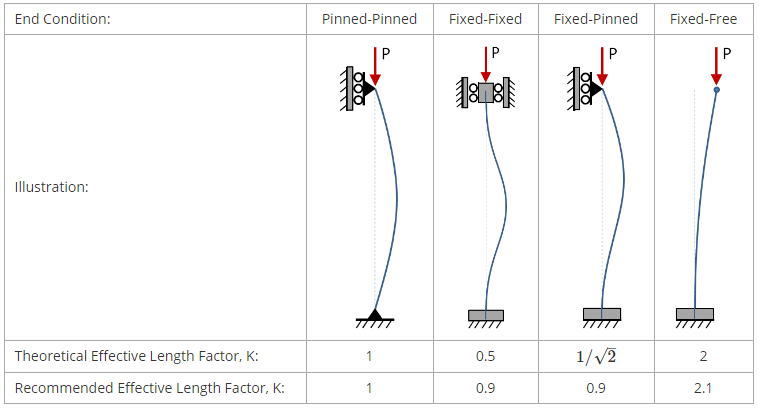
\includegraphics[width=1.0\textwidth]{figures/endcondpipe.PNG}
\caption{End conditions of pipe \cite{buckling}}
\label{fig:endcondpipe}
\end{figure}

Due to the implementation of a riser above the formation, the end conditions will be \textit{fixed-fixed}, which yields a recommended effective length factor, $K$, of 0.9.

Input data for equation (\ref{eq:eulerbuckling}) can be found in table (\ref{tab:inputdataeuler})


\begin{table} [H]
    \centering
    \caption{Input data for Euler's Critcal Load}
    \begin{tabular}{p{2cm} p{3cm}}
        E [Pa] & $6.9\cdot10^{10}$ \\ \hline
        I [m$^4$] & $2.27\cdot10^{-10}$ \\ \hline
        K & $0.9$ \\ \hline
        L [m] & $0.91$ \\ 
    \end{tabular}
    \label{tab:inputdataeuler}
\end{table}

The critical load was found to be 230.7 N, equivalent to a weight of 23.5 kg. This means that when the internal pressure is increased using the nozzle in the BHA, the pipe will enter a state of compression when the WOB passes 31.0 kg, but it will not, based on this estimation buckle until it reaches the sum of F$_c$, the drill string weight and the critical load, in this case 50 kg.

The goal will still be to avoid putting the string in compression, but if it becomes clear during phase II that a WOB of 31.0 kg is insufficient to drill efficiently, it will be considered whether a higher WOB can be used or not.

\subsection{Drill String Compression Analysis Results} \caption{ssec:comp}

\begin{table} [H]
    \centering
    \caption{Estimated values for Fc, weight of drill string and maximum WOB.}
    \begin{tabular}{p{5cm} p{2cm}}
        $F_c$ [kg] & 31.0 \\ \hline
        Weight of Drill String [kg] & 0.5 \\ \hline
        Maximum WOB [kg] & 31.5 \\ \hline
        Critical WOB [kg] & 50.0 \\ \hline
    \end{tabular}
    \label{tab:summarywob}
\end{table}

A total of 31.5 kg can be applied on the drill string through the top drive while maintaining the neutral point in the BHA when using a constriction with a flow diameter of 1.38 mm in the BHA.

